\documentclass[]{informeutn}

\addbibresource{fuentes.bib}
\usepackage{csquotes}
\usepackage{amssymb}
\usepackage{subcaption}
\usepackage[section]{placeins}

% --- Configuración de la Carátula ---
\titulo{Trabajo Práctico N° 4}
\subtitulo{Muestreo, Recuperación de Señales y Codificación PCM}
\materia{Sistemas de Comunicaciones}
\comision{4R2}
\autores{
    Grasso, Gaston - 401892\\
    Palombo, Franco - 401910\\
    Prieto, Angelo - 401012\\[1em]
    \textbf{Docente:} Ing. Sergio Brandan
}
\fecha{2024}

\begin{document}
  \maketitle
  
  \tableofcontents
  \setcounter{page}{1}
  \thispagestyle{plain}

  \chapter{Introducción y Objetivos}
\label{sec.ej4:introduccion}

El presente trabajo práctico aborda la simulación y análisis del proceso de muestreo y recuperación analógica de una
señal en banda base, así como la simulación de un sistema de codificación por modulación de impulsos codificados (PCM).

\section{Objetivos}
De acuerdo con la consigna, los objetivos fijados para la actividad son:
\begin{itemize}
    \item Realizar una simulación del proceso de muestreo y recuperación de una señal analógica mediante filtrado
          pasabajos.
    \item Validar la frecuencia de muestreo de acuerdo con el criterio de Nyquist.
    \item Mostrar y caracterizar el efecto de solapamiento espectral (aliasing) en el dominio temporal y frecuencial.
    \item Analizar el concepto de expansión del espectro derivado del muestreo.
    \item Determinar por qué el teorema resulta en una modulación de pulsos (PAM).
    \item Analizar el cuasi-muestreo a partir de muestrear con una portadora sin componente continua.
    \item Realizar una simulación de codificación PCM de una señal, verificando el comportamiento temporal en el bus
          paralelo de salida del convertidor y en la trama serie multiplexada.
\end{itemize}

\section{Esquemas de Implementación y Parámetros Fijados}
El desarrollo se estructuró a partir de dos esquemas de simulación en NI Multisim:
\begin{enumerate}
    \item \textbf{Muestreo y Recuperación de Señal:} La señal de banda base (punto A) se combina con la señal
          muestreadora (punto B) en un bloque muestreador para obtener la señal muestreada (punto C), la cual ingresa a
          una etapa de recuperación por filtrado pasabajos para obtener la señal analógica recuperada (punto D).
          Los valores de implementación fijados son:
          \begin{itemize}
              \item Señal de banda base: senoidal de $1\,\unit{\volt}$ de amplitud pico y frecuencia $10\,\unit{\kilo\hertz}$.
              \item Señal muestreadora: tren de pulsos con frecuencia nominal de $40\,\unit{\kilo\hertz}$.
          \end{itemize}
    \item \textbf{Sistema de Codificación PCM:} La señal analógica de entrada se muestrea y cuantiza mediante un
          conversor analógico-digital (ADC) de 8 bits, entregando la palabra binaria paralela en el punto de medición G.
          Dicha palabra se ingresa a un multiplexor digital para serializar los bits y obtener la trama binaria serie
          en el punto de medición H.
\end{enumerate}

  \FloatBarrier
  \chapter{Muestreo y Recuperación de una Señal}
\label{sec.ej4:muestreo}

En este capítulo se analiza la simulación del proceso de muestreo natural y recuperación analógica por filtrado
pasabajos, respondiendo puntualmente a cada uno de los ítems de desarrollo solicitados en la consigna.

\section{Circuito Implementado}
En la figura \ref{crkt.ej4:muestreo} se presenta el circuito implementado en NI Multisim para este ensayo.

\begin{figure}[!ht]
    \centering
    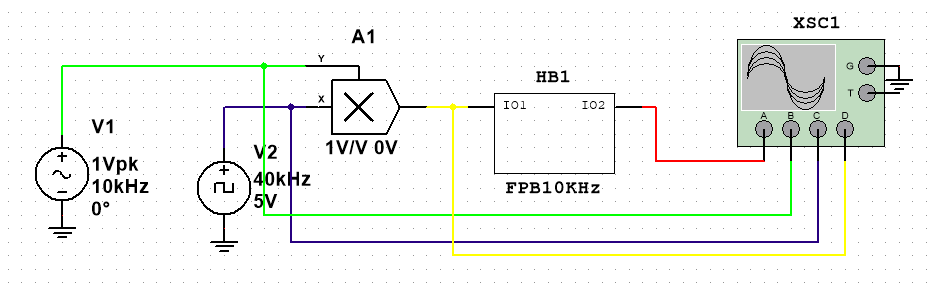
\includegraphics[width=0.75\textwidth]{images/muestreo_circuito.png}
    \caption{Circuito de simulación para muestreo natural y recuperación por filtrado pasabajos.}
    \label{crkt.ej4:muestreo}
\end{figure}

El circuito se compone de:
\begin{itemize}
    \item Generador de señal senoidal $V_1$: fija la señal en banda base en el punto A con $1\,\unit{\volt}$ de pico y
          frecuencia $f_m = 10\,\unit{\kilo\hertz}$.
    \item Generador de pulsos de muestreo $V_2$: introduce en el punto B el tren de pulsos rectangulares con frecuencia
          nominal $f_s = 40\,\unit{\kilo\hertz}$, amplitud de $5\,\unit{\volt}$ y ciclo de trabajo del $50\%$.
    \item Multiplicador analógico $A_1$: efectúa el producto analógico entre ambas señales ($k = 1\,\unit{\volt/\volt}$),
          obteniéndose en su salida (punto C) la señal muestreada.
    \item Filtro pasabajos de reconstrucción $HB_1$ (FPB10KHz): bloque de filtrado activo con frecuencia de corte
          nominal de $10\,\unit{\kilo\hertz}$, en cuya salida (punto D) se obtiene la señal analógica recuperada.
    \item Osciloscopio digital $XSC_1$: conectado a los puntos A (Canal B), B (Canal C), C (Canal D) y D (Canal A).
\end{itemize}

\section{Validación de la Frecuencia de Muestreo}
El Teorema de Nyquist-Shannon establece que la frecuencia de muestreo $f_s$ debe satisfacer la condición:
\begin{equation}
    f_s \ge 2 f_{\max}
    \label{eq.ej4:nyquist}
\end{equation}
Para la señal de banda base de frecuencia $f_m = 10\,\unit{\kilo\hertz}$, la frecuencia mínima de muestreo requerida es:
\begin{equation*}
    f_{s,\mathrm{Nyq}} = 2 \cdot 10\,\unit{\kilo\hertz} = 20\,\unit{\kilo\hertz}
\end{equation*}
La frecuencia adoptada en la implementación es $f_s = 40\,\unit{\kilo\hertz}$, la cual duplica el límite teórico de
Nyquist ($40\,\unit{\kilo\hertz} > 20\,\unit{\kilo\hertz}$). Esta elección proporciona una banda de guarda espectral:
\begin{equation}
    B_g = (f_s - f_m) - f_m = (40 - 10)\,\unit{\kilo\hertz} - 10\,\unit{\kilo\hertz} = 20\,\unit{\kilo\hertz}
    \label{eq.ej4:banda_guarda}
\end{equation}
La presencia de este margen de $20\,\unit{\kilo\hertz}$ asegura que el filtro pasabajos de corte en $10\,\unit{\kilo\hertz}$
atenúe adecuadamente la primera banda lateral inferior en $30\,\unit{\kilo\hertz}$, permitiendo recuperar la señal
senoidal en el punto D sin distorsión.

\section{Resumen Temporal en los Puntos A, B, C y D}
En la figura \ref{fig.ej4:muestreo_40k_temporal} se muestran las formas de onda registradas por el osciloscopio virtual
para la condición $f_s = 40\,\unit{\kilo\hertz}$.

\begin{figure}[!ht]
    \centering
    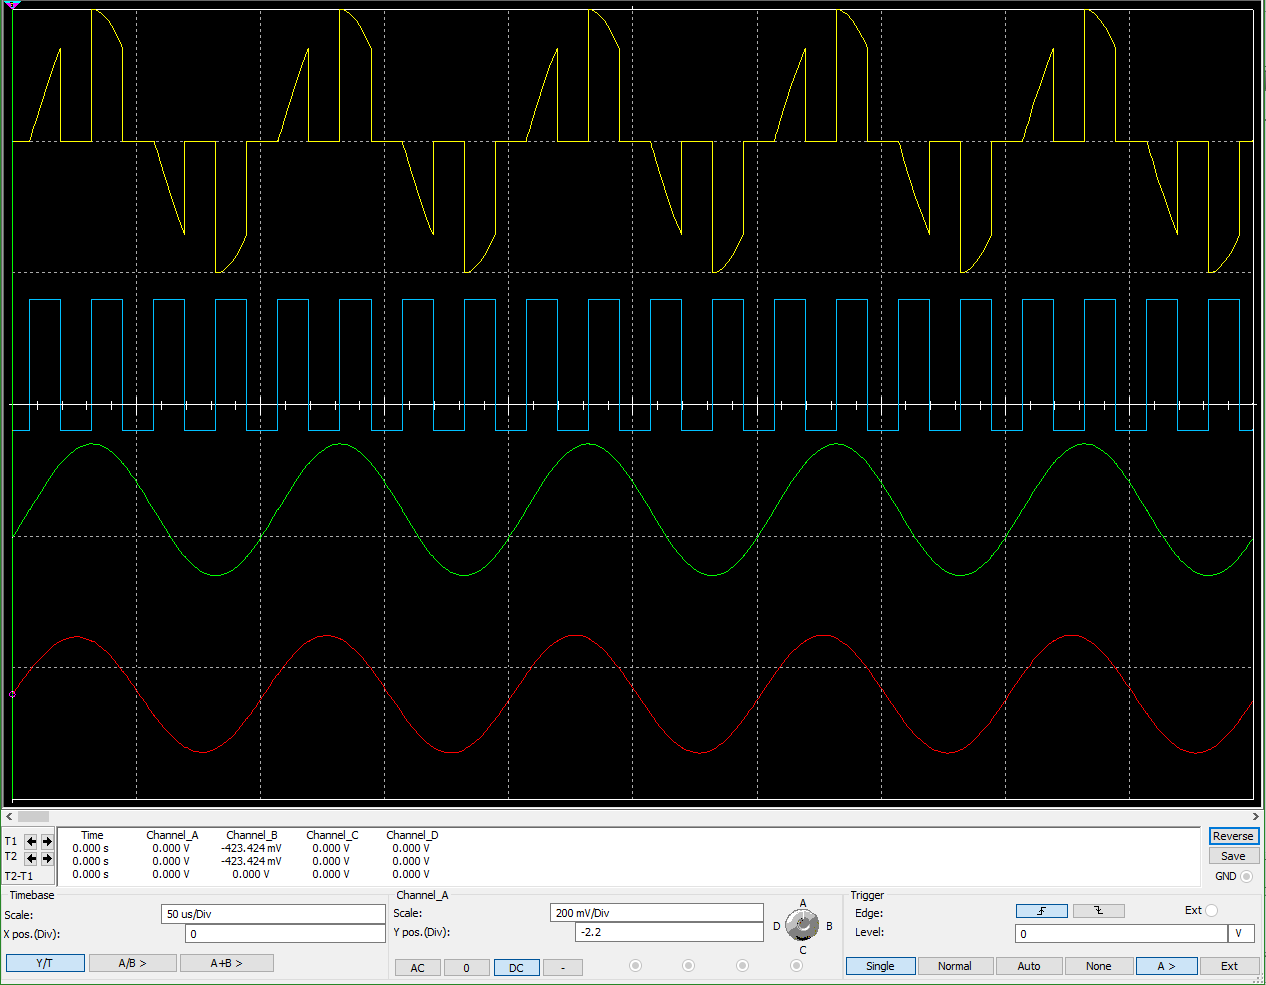
\includegraphics[width=0.75\textwidth]{images/muestreo_40khz_temporal.png}
    \caption{Formas de onda temporales con $f_s = 40\,\unit{\kilo\hertz}$: señal modulante (punto A, verde), tren de
             muestreo (punto B, azul), señal PAM natural (punto C, amarillo) y señal recuperada (punto D, rojo).}
    \label{fig.ej4:muestreo_40k_temporal}
\end{figure}

Las mediciones temporales verifican:
\begin{itemize}
    \item \textbf{Punto A (Canal B, verde):} Senoidal pura de $1\,\unit{\volt}$ de amplitud y período
          $T_m = 1/10\,\unit{\kilo\hertz} = 100\,\unit{\micro\second}$.
    \item \textbf{Punto B (Canal C, azul):} Tren de pulsos rectangulares de $0$ a $5\,\unit{\volt}$ con período
          $T_s = 1/40\,\unit{\kilo\hertz} = 25\,\unit{\micro\second}$. Se registran exactamente 4 pulsos por ciclo de la
          señal modulante.
    \item \textbf{Punto C (Canal D, amarillo):} Señal muestreada PAM natural. Durante el intervalo en que el pulso está
          en alto, la señal sigue la forma senoidal instantánea de la entrada; durante el nivel bajo del pulso, cae a cero.
    \item \textbf{Punto D (Canal A, rojo):} Señal senoidal pura recuperada a la salida del filtro pasabajos, libre de
          ondulación de conmutación y con el retardo temporal propio de la respuesta de fase del filtro.
\end{itemize}

\section{Análisis de la Expansión del Espectro}
La multiplicación temporal de la señal de entrada $x(t)$ por el tren de pulsos periódico $p(t)$ equivale en frecuencia
a la convolución de sus respectivos espectros:
\begin{equation}
    S(f) = X(f) * P(f) = \sum_{n=-\infty}^\infty c_n X(f - n f_s)
    \label{eq.ej4:convolucion}
\end{equation}
donde $c_n$ son los coeficientes de Fourier del tren de pulsos.

Como el tren de conmutación posee armónicos en múltiplos enteros de la frecuencia de muestreo ($n f_s$), el espectro
de la señal de entrada (confinado a $10\,\unit{\kilo\hertz}$) se replica alrededor de cada armónico $n f_s$, generando
bandas laterales en $n f_s \pm f_m$. Esto produce una expansión del espectro, ya que la energía de la señal deja de estar
restringida a la banda base y se propaga teóricamente hacia frecuencias infinitas, modulada por la envolvente sinc
propia del ancho finito de los pulsos.

Este fenómeno se comprobó en la simulación mediante las mediciones por FFT:
\begin{itemize}
    \item En la figura \ref{fig.ej4:fft_entrada_40k} se observa el espectro de entrada en el punto A, con un único tono
          puro en $10\,\unit{\kilo\hertz}$.
    \item En la figura \ref{fig.ej4:fft_muestreo_40k} se observa el espectro de la señal muestreada en el punto C,
          evidenciando la expansión espectral con componentes en $f_m = 10\,\unit{\kilo\hertz}$, $f_s - f_m = 30\,\unit{\kilo\hertz}$,
          $f_s = 40\,\unit{\kilo\hertz}$, $f_s + f_m = 50\,\unit{\kilo\hertz}$ y armónicos superiores.
    \item En la figura \ref{fig.ej4:fft_salida_40k} se verifica la acción del filtro pasabajos en el punto D, el cual
          elimina todas las réplicas espectrales superiores y restituye de forma limpia el tono de $10\,\unit{\kilo\hertz}$.
\end{itemize}

\begin{figure}[!ht]
    \centering
    \begin{subfigure}[t]{0.32\textwidth}
        \centering
        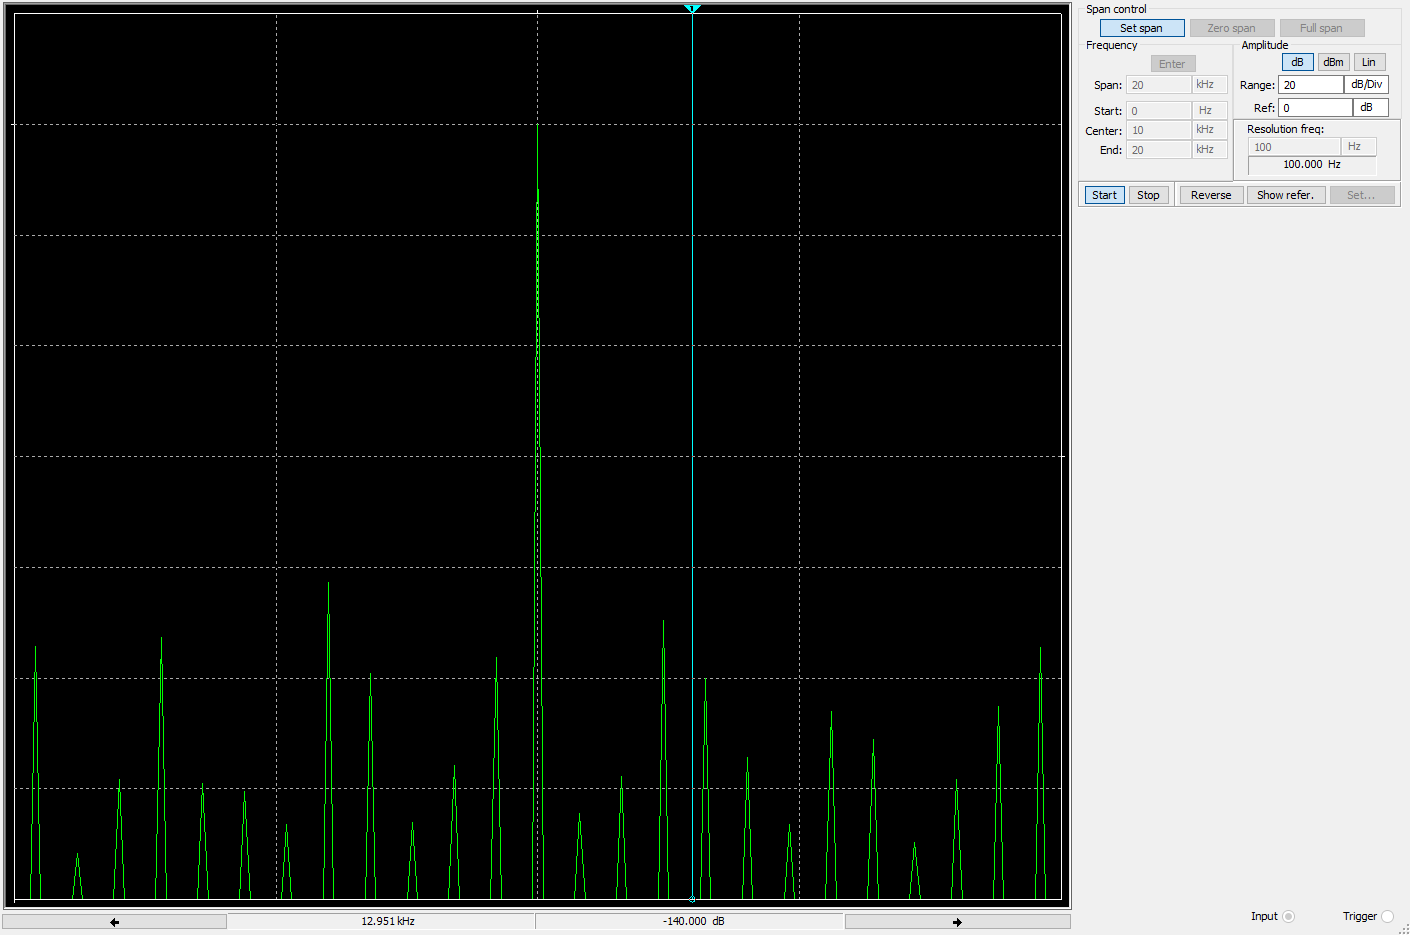
\includegraphics[width=\textwidth]{images/fft_entrada_40khz.png}
        \caption{Tono de entrada (punto A).}
        \label{fig.ej4:fft_entrada_40k}
    \end{subfigure}\hfill
    \begin{subfigure}[t]{0.32\textwidth}
        \centering
        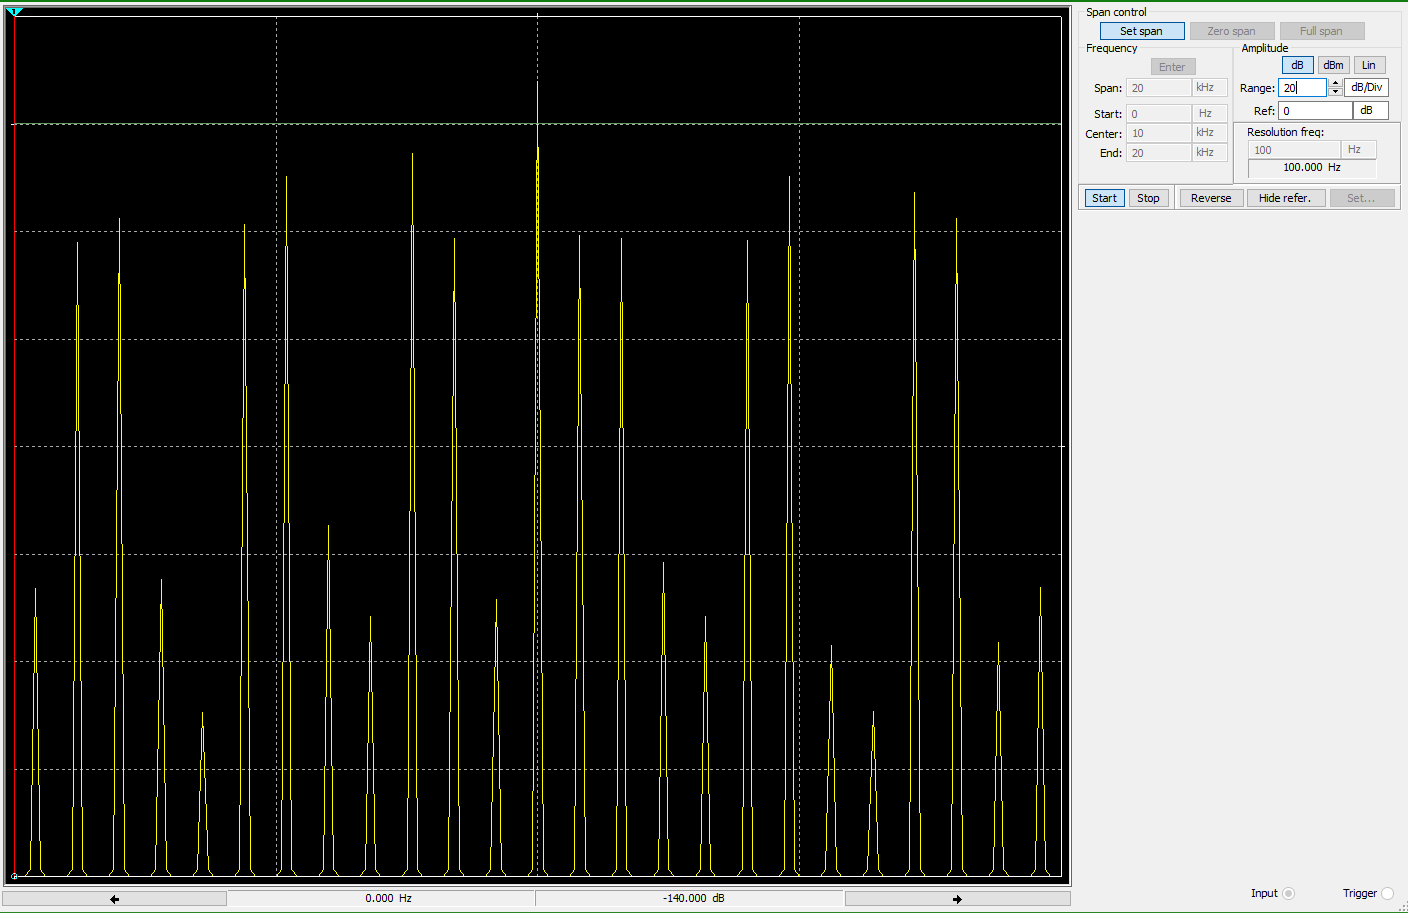
\includegraphics[width=\textwidth]{images/fft_muestreo_40khz.png}
        \caption{Señal PAM (punto C).}
        \label{fig.ej4:fft_muestreo_40k}
    \end{subfigure}\hfill
    \begin{subfigure}[t]{0.32\textwidth}
        \centering
        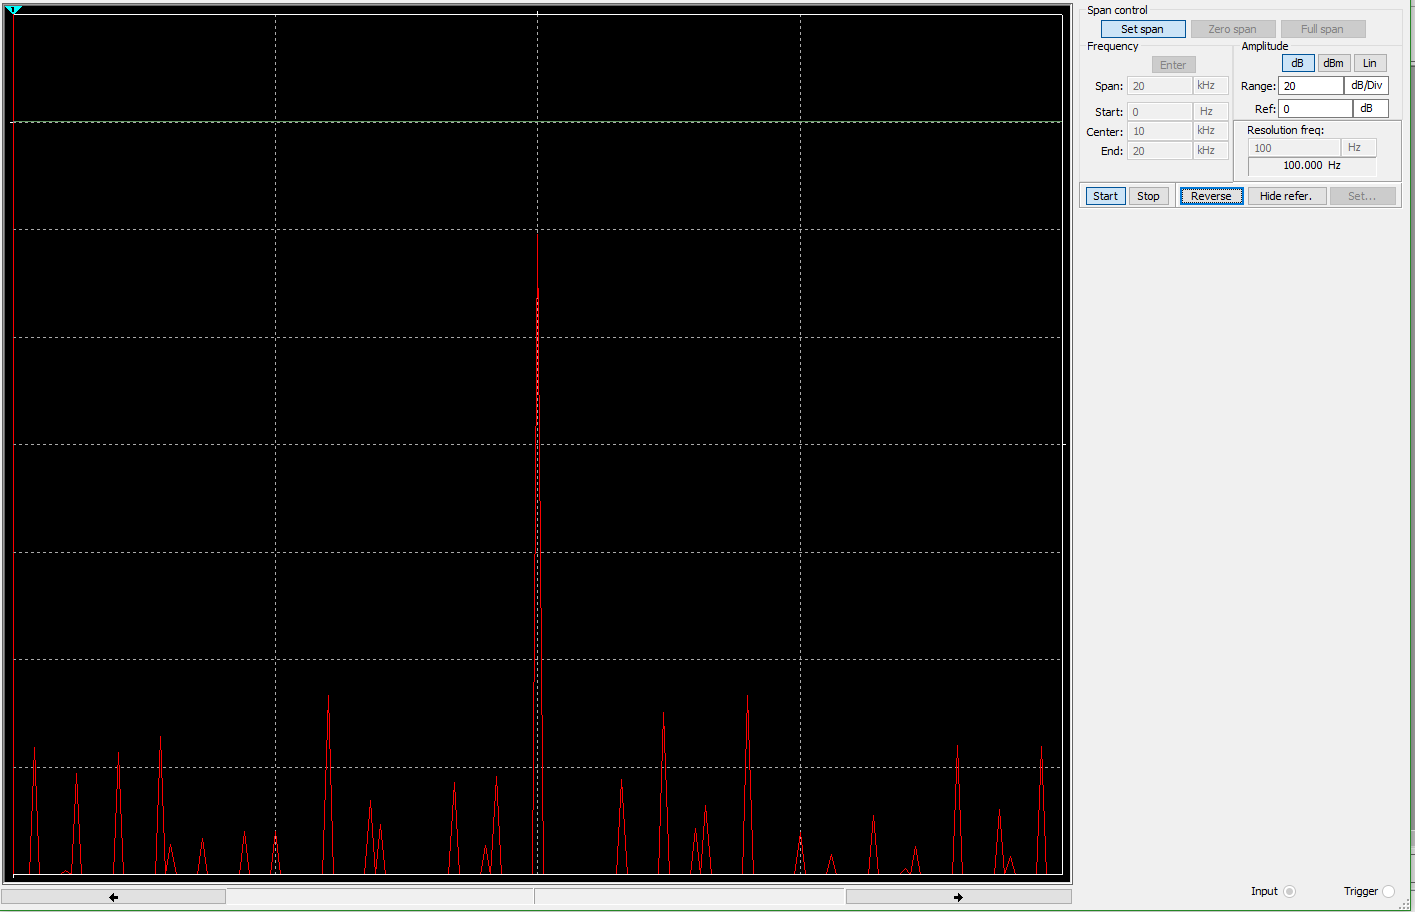
\includegraphics[width=\textwidth]{images/fft_salida_40khz.png}
        \caption{Recuperada (punto D).}
        \label{fig.ej4:fft_salida_40k}
    \end{subfigure}
    \caption{Evolución espectral FFT con $f_s = 40\,\unit{\kilo\hertz}$ en los puntos A, C y D.}
    \label{fig.ej4:fft_evolucion_40k}
\end{figure}

\section{Determinación de por qué el Teorema Resulta en una Modulación de Pulsos}
El teorema del muestreo implementado físicamente a través de una llave conmutadora o multiplicador analógico responde a
una modulación de pulsos en amplitud (PAM).

Desarrollando el tren de pulsos unipolar en serie trigonométrica de Fourier:
\begin{equation}
    p(t) = a_0 + \sum_{n=1}^\infty a_n \cos(n \omega_s t)
    \label{eq.ej4:fourier_tren}
\end{equation}
donde $a_0 = V_p d$ y $a_n = 2 V_p d \operatorname{sinc}(n \pi d)$. Al multiplicar por la señal modulante
$x(t) = A_m \cos(\omega_m t)$:
\begin{equation}
    s(t) = a_0 x(t) + \sum_{n=1}^\infty \frac{a_n A_m}{2} \left[ \cos\left((n \omega_s - \omega_m)t\right) + \cos\left((n \omega_s + \omega_m)t\right) \right]
    \label{eq.ej4:pam_desarrollo}
\end{equation}
La ecuación (\ref{eq.ej4:pam_desarrollo}) explica por qué el proceso constituye una modulación de pulsos:
\begin{enumerate}
    \item En el dominio del tiempo, la amplitud de cada pulso rectangular es modulada linealmente por la magnitud
          instantánea de la señal continua de entrada.
    \item En el dominio de la frecuencia, cada armónico $n \omega_s$ del tren periódico actúa como una portadora
          independiente que es modulada en amplitud (doble banda lateral) por la señal de información en banda base.
    \item La existencia de la componente continua $a_0$ garantiza que el espectro contenga una réplica directa de la
          señal modulante $a_0 x(t)$ en el origen, permitiendo recuperarla con un filtro pasabajos lineal.
\end{enumerate}

\section{Demostración del Efecto de Aliasing}
Para constatar el efecto de aliasing o solapamiento espectral, se reconfiguró la frecuencia de muestreo a
$f_s = 15\,\unit{\kilo\hertz}$, manteniéndose $f_m = 10\,\unit{\kilo\hertz}$ y el filtro pasabajos de $10\,\unit{\kilo\hertz}$.

Bajo esta condición se viola el criterio de Nyquist, ya que la frecuencia de muestreo es menor que el doble de la
frecuencia de la modulante:
\begin{equation*}
    f_s = 15\,\unit{\kilo\hertz} < 2 f_m = 20\,\unit{\kilo\hertz}
\end{equation*}
La frecuencia de Nyquist (frecuencia de plegamiento) se reduce a $f_N = f_s / 2 = 7{,}5\,\unit{\kilo\hertz}$. Como la
señal de $10\,\unit{\kilo\hertz}$ excede $f_N$, la primera banda lateral inferior se repliega hacia la banda base en:
\begin{equation}
    f_{\mathrm{alias}} = |f_s - f_m| = |15 - 10|\,\unit{\kilo\hertz} = 5{,}0\,\unit{\kilo\hertz}
    \label{eq.ej4:f_alias}
\end{equation}
Dado que el filtro pasabajos posee corte en $10\,\unit{\kilo\hertz}$, la componente espuria de $5\,\unit{\kilo\hertz}$
cae dentro de su banda de paso ($5\,\unit{\kilo\hertz} < 10\,\unit{\kilo\hertz}$). En consecuencia, el filtro deja pasar
simultáneamente la señal deseada de $10\,\unit{\kilo\hertz}$ y el alias de $5\,\unit{\kilo\hertz}$.

En la figura \ref{fig.ej4:aliasing_15k_completo} se presenta la verificación del fenómeno en el dominio del tiempo
y en frecuencia. En el osciloscopio (figura \ref{fig.ej4:muestreo_15k_temporal}) se aprecia el impacto temporal: la
señal recuperada en el punto D (rojo) resulta fuertemente distorsionada, exhibiendo un batido periódico con frecuencia
$f_{\mathrm{batido}} = 10 - 5 = 5\,\unit{\kilo\hertz}$ ($T_{\mathrm{batido}} = 200\,\unit{\micro\second}$, correspondiente
a 4 divisiones horizontales de $50\,\unit{\micro\second/\mathrm{div}}$). En el analizador de espectro (figura
\ref{fig.ej4:fft_salida_15k}) se constatan simultáneamente el tono fundamental en $10\,\unit{\kilo\hertz}$ y la raya
espuria de aliasing en $5\,\unit{\kilo\hertz}$, confirmando la degradación irreversible de la señal analógica.

\begin{figure}[!ht]
    \centering
    \begin{subfigure}[t]{0.48\textwidth}
        \centering
        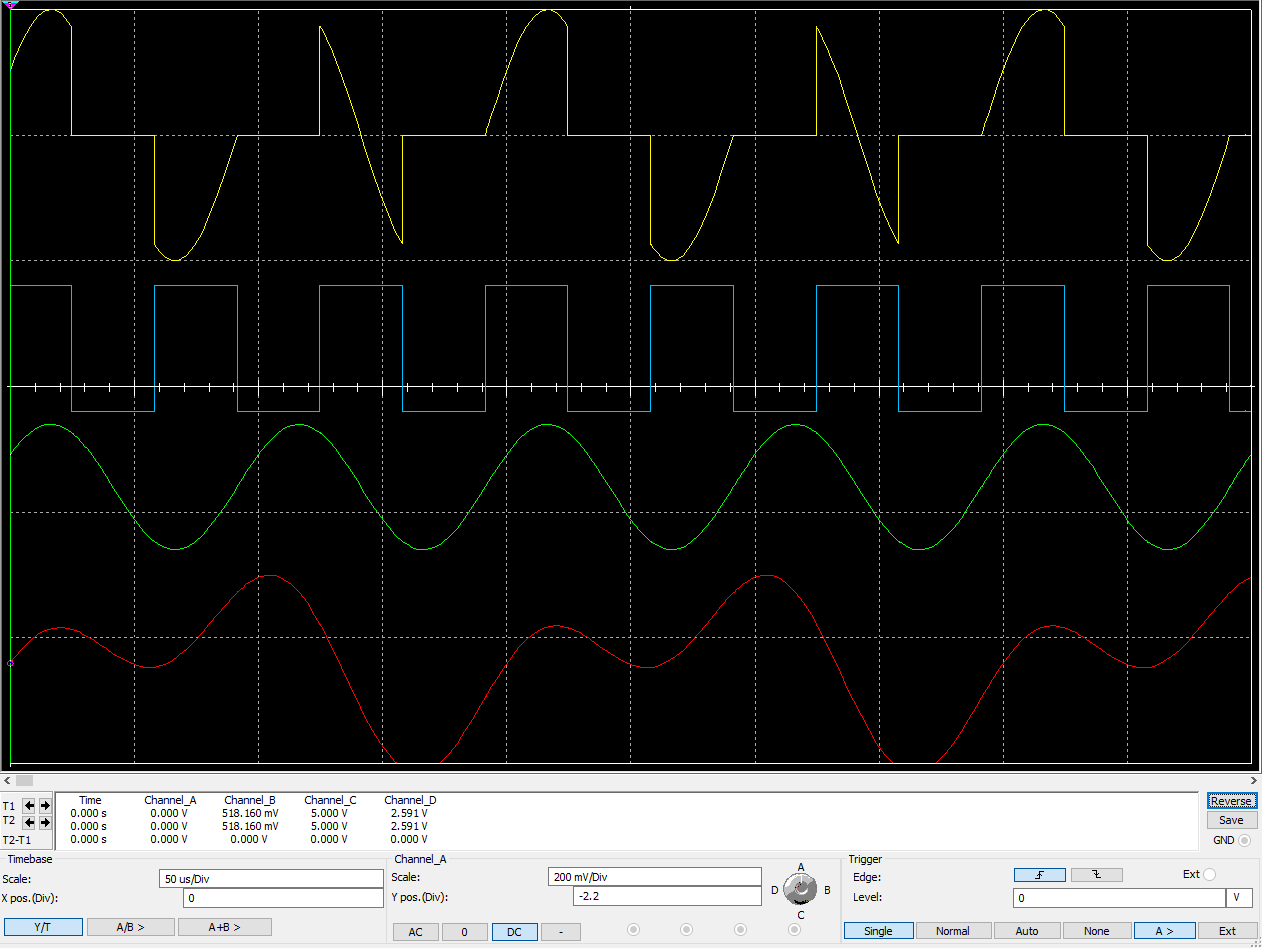
\includegraphics[width=\textwidth]{images/muestreo_15khz_aliasing_temporal.png}
        \caption{Dominio del tiempo: batido y distorsión en D.}
        \label{fig.ej4:muestreo_15k_temporal}
    \end{subfigure}\hfill
    \begin{subfigure}[t]{0.48\textwidth}
        \centering
        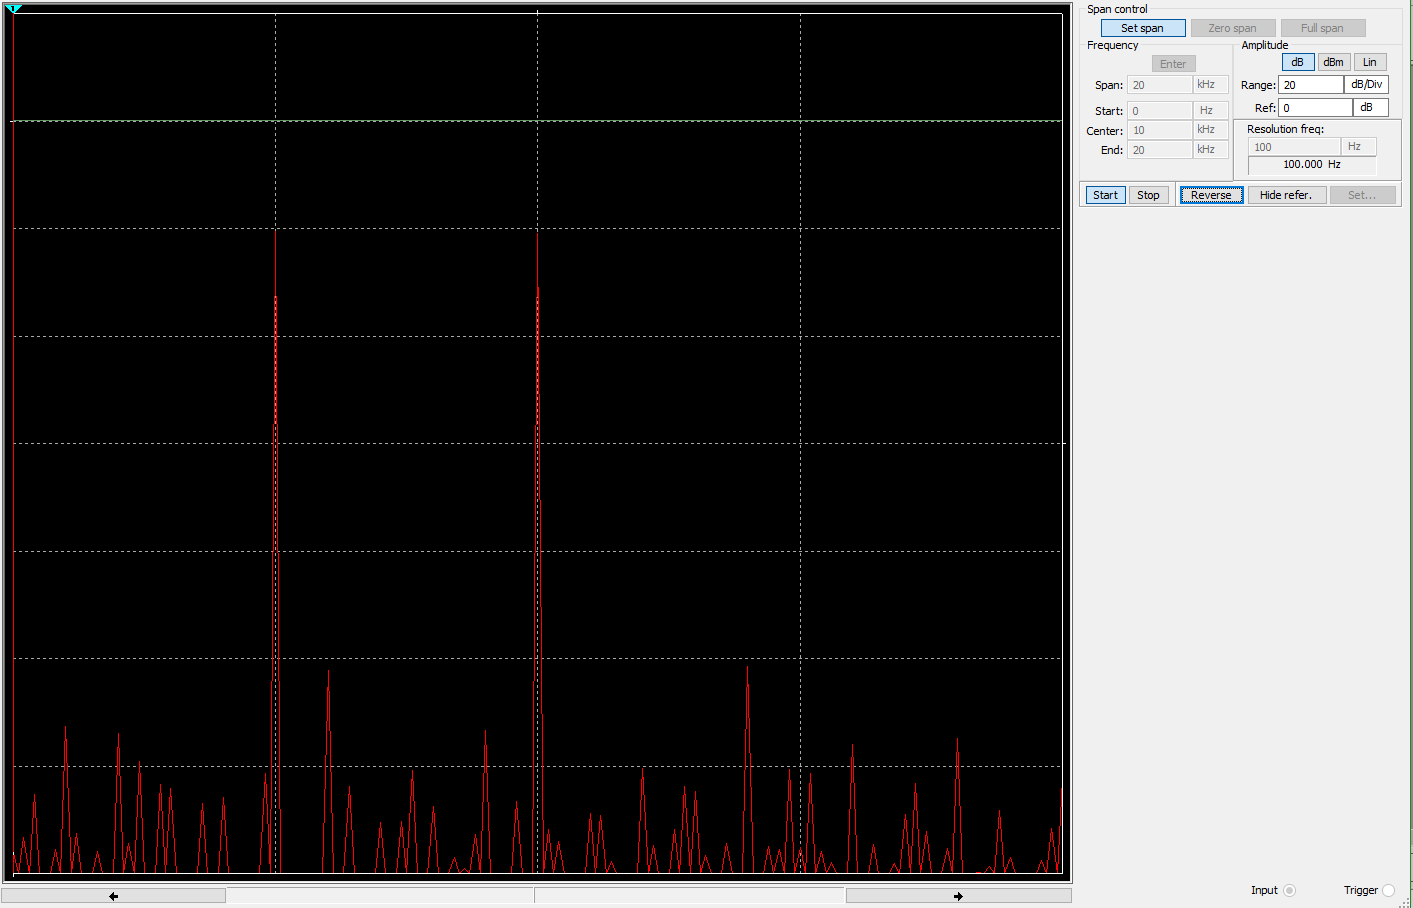
\includegraphics[width=\textwidth]{images/fft_salida_15khz_aliasing.png}
        \caption{Dominio frecuencial: raya alias en $5\,\unit{\kilo\hertz}$.}
        \label{fig.ej4:fft_salida_15k}
    \end{subfigure}
    \caption{Efecto de Aliasing para $f_s = 15\,\unit{\kilo\hertz}$ en tiempo y frecuencia.}
    \label{fig.ej4:aliasing_15k_completo}
\end{figure}

\section{Análisis del Cuasi-Muestreo sin Componente Continua}
El cuasi-muestreo se analizó configurando la señal de conmutación como una onda cuadrada bipolar simétrica oscilando
entre $+2{,}5\,\unit{\volt}$ y $-2{,}5\,\unit{\volt}$ con $f_s = 40\,\unit{\kilo\hertz}$ y ciclo de trabajo del $50\%$.
Bajo esta condición, el valor medio del tren de conmutación es nulo ($a_0 = 0$).

La serie de Fourier de una onda cuadrada bipolar simétrica carece de término de continua y de armónicos pares:
\begin{equation}
    p_{\mathrm{bip}}(t) = \frac{4 V_p}{\pi} \sum_{k=1, 3, 5, \dots}^\infty \frac{(-1)^{(k-1)/2}}{k} \cos(k \omega_s t)
    \label{eq.ej4:fourier_bipolar}
\end{equation}
Al multiplicar por la entrada $x(t) = A_m \cos(\omega_m t)$:
\begin{equation}
    s(t) = \sum_{k=1, 3, \dots}^\infty \frac{2 A_m V_p}{\pi k} (-1)^{(k-1)/2} \left[ \cos\left((k \omega_s - \omega_m)t\right) + \cos\left((k \omega_s + \omega_m)t\right) \right]
    \label{eq.ej4:producto_bipolar}
\end{equation}
El resultado de la ecuación (\ref{eq.ej4:producto_bipolar}) demuestra que:
\begin{itemize}
    \item \textbf{No existe componente en banda base:} Al anularse $a_0$, no hay ningún término en $f_m = 10\,\unit{\kilo\hertz}$.
    \item \textbf{Modulación DSB-SC:} La señal producto contiene únicamente bandas laterales alrededor
          de armónicos impares de conmutación. La frecuencia más baja es $f_s - f_m = 40 - 10 = 30\,\unit{\kilo\hertz}$.
    \item \textbf{Anulación de la salida recuperada:} Como la componente más baja ($30\,\unit{\kilo\hertz}$) se ubica muy
          por encima de la frecuencia de corte del filtro pasabajos ($10\,\unit{\kilo\hertz}$), el filtro la atenúa por
          completo, resultando en una salida de $0\,\unit{\volt}$ en el punto D.
\end{itemize}

En la figura \ref{fig.ej4:cuasi_muestreo_completo} se presenta la verificación temporal y espectral: en el
osciloscopio (figura \ref{fig.ej4:muestreo_sin_cc_temporal}) la señal recuperada en el punto D (trazo rojo) se anula
por completo ($1{,}55\,\unit{\micro\volt}$ residuales de simulación). En el analizador de espectro (figura
\ref{fig.ej4:fft_muestreo_sin_cc}) se comprueba la ausencia absoluta de energía en $10\,\unit{\kilo\hertz}$. Por lo
tanto, muestrear sin componente continua no produce muestreo en banda base recuperable por filtrado lineal, sino una
modulación balanceada en doble banda lateral con portadora suprimida que requiere demodulación coherente.

\begin{figure}[!ht]
    \centering
    \begin{subfigure}[t]{0.48\textwidth}
        \centering
        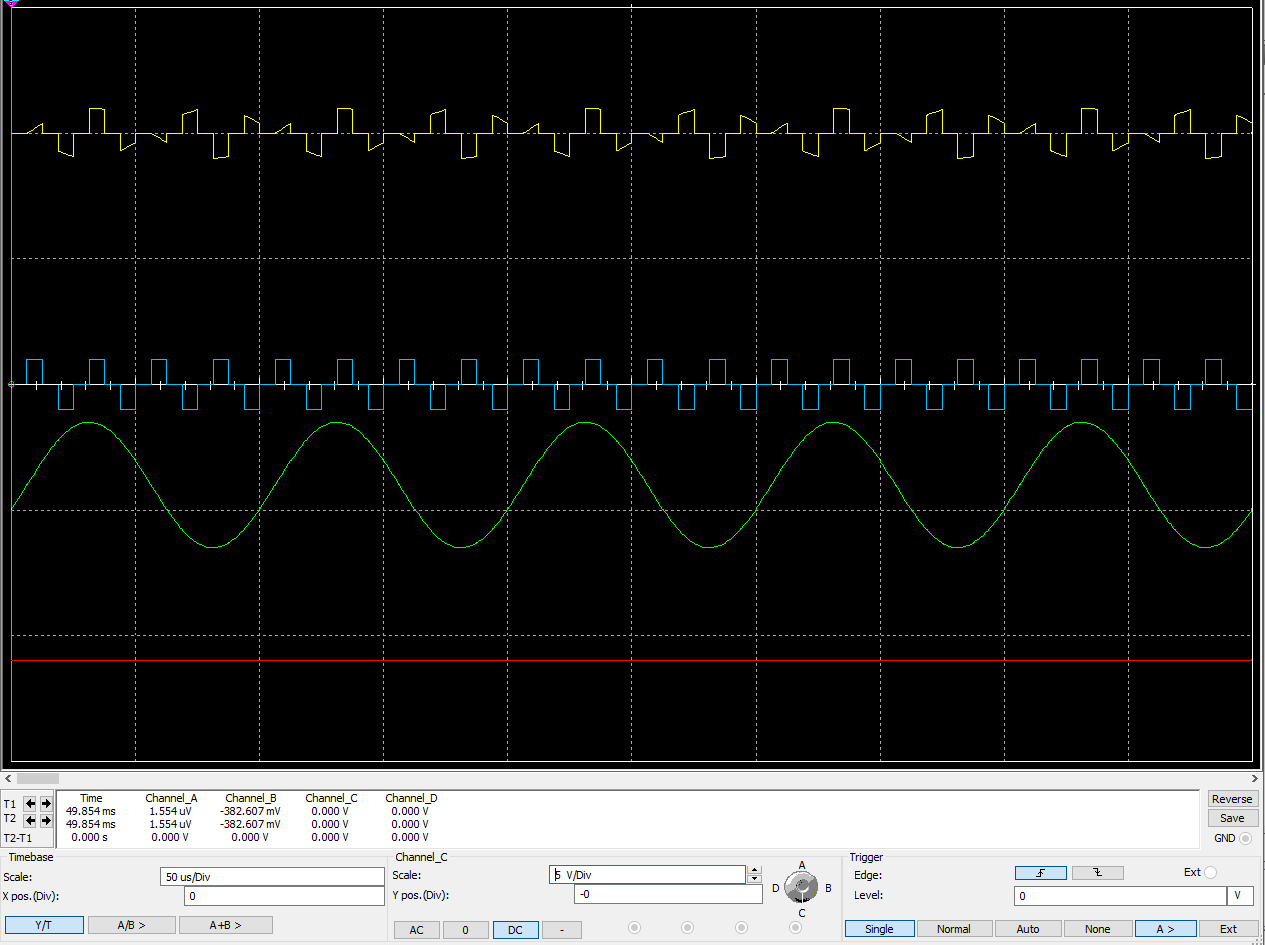
\includegraphics[width=\textwidth]{images/muestreo_sin_cc_temporal.png}
        \caption{Dominio del tiempo: salida D nula en $0\,\unit{\volt}$.}
        \label{fig.ej4:muestreo_sin_cc_temporal}
    \end{subfigure}\hfill
    \begin{subfigure}[t]{0.48\textwidth}
        \centering
        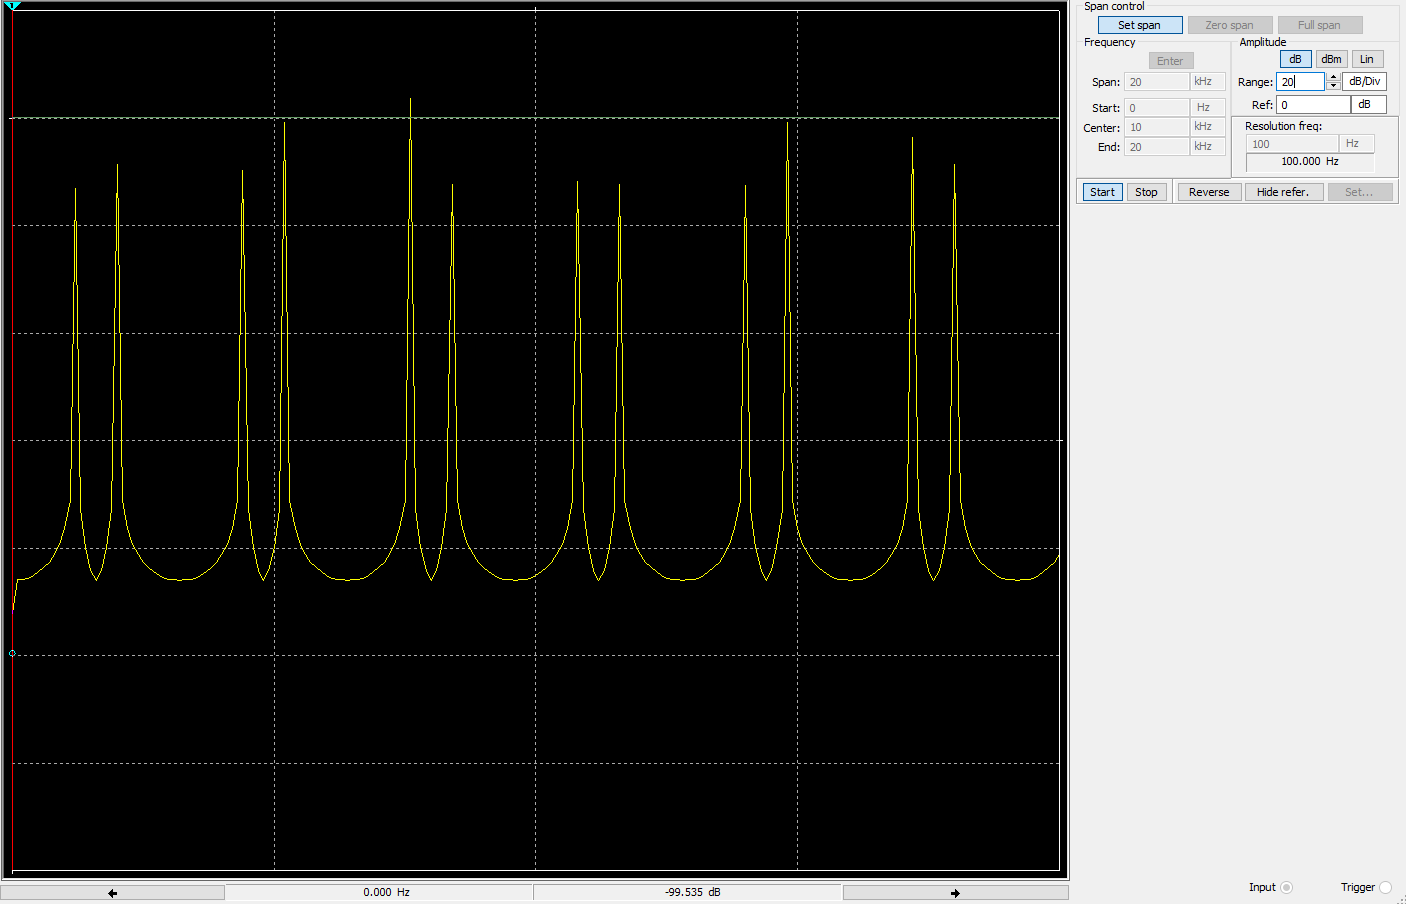
\includegraphics[width=\textwidth]{images/fft_muestreo_sin_cc.png}
        \caption{Dominio frecuencial: ausencia de banda base.}
        \label{fig.ej4:fft_muestreo_sin_cc}
    \end{subfigure}
    \caption{Cuasi-muestreo sin componente continua ($a_0 = 0$) en tiempo y frecuencia.}
    \label{fig.ej4:cuasi_muestreo_completo}
\end{figure}

  \FloatBarrier
  \chapter{Sistema de Codificación PCM}
\label{sec.ej4:pcm}

En este capítulo se analiza la simulación del sistema de digitalización y codificación PCM de acuerdo con el segundo
esquema establecido en la consigna.

\section{Circuito Implementado}
En la figura \ref{crkt.ej4:digitalizacion} se presenta el circuito implementado en NI Multisim para la codificación y
serialización PCM.

\begin{figure}[!ht]
    \centering
    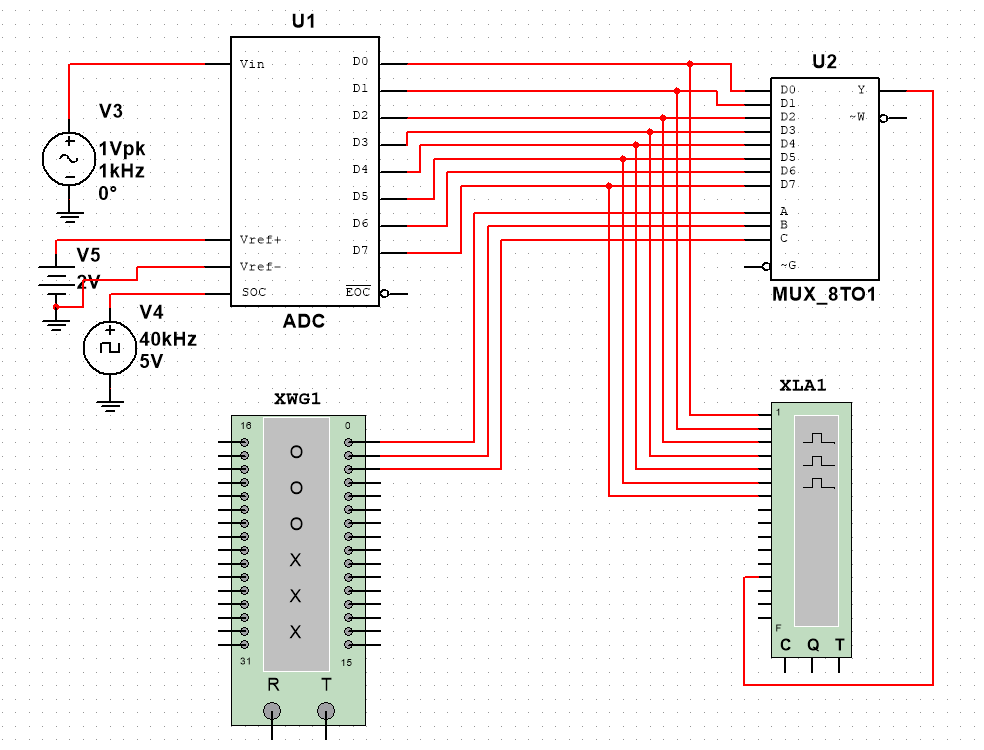
\includegraphics[width=0.75\textwidth]{images/digitalizacion_circuito.png}
    \caption{Circuito del sistema de codificación PCM con ADC de 8 bits, multiplexor 8 a 1, generador de palabras y
             analizador lógico.}
    \label{crkt.ej4:digitalizacion}
\end{figure}

El sistema está conformado por los siguientes bloques:
\begin{itemize}
    \item Fuente senoidal de entrada $V_3$: señal analógica de $1\,\unit{\volt_\mathrm{pk}}$ y frecuencia de $1\,\unit{\kilo\hertz}$.
    \item Conversor analógico-digital $U_1$ (ADC): convertidor de 8 bits alimentado con tensiones de referencia
          $V_{\mathrm{ref}+} = 2{,}0\,\unit{\volt}$ y $V_{\mathrm{ref}-} = 0{,}0\,\unit{\volt}$.
    \item Reloj de muestreo $V_4$: tren de pulsos de $5\,\unit{\volt}$ y frecuencia $f_s = 40\,\unit{\kilo\hertz}$
          conectado al terminal SOC (Start Of Conversion) para gobernar la cadencia de muestreo del ADC.
    \item Multiplexor digital $U_2$ (MUX\_8TO1): dispositivo selector de 8 canales a 1 salida, cuyas entradas de datos
          se conectan a las salidas paralelas del convertidor.
    \item Generador de palabras digitales (XWG1): provee una secuencia cíclica ascendente de 3 bits ($000_2$ a $111_2$)
          conectada a las líneas de dirección A, B y C del multiplexor para serializar la palabra binaria dentro de cada
          período de muestreo.
    \item Analizador lógico (XLA1): registra en forma sincrónica las líneas paralelas del ADC y la salida serializada.
\end{itemize}

A partir de los valores del circuito, los parámetros característicos de la digitalización resultan:
\begin{itemize}
    \item Fondo de escala: $V_{\mathrm{FSR}} = V_{\mathrm{ref}+} - V_{\mathrm{ref}-} = 2{,}0\,\unit{\volt}$.
    \item Cantidad de niveles discretos: $L = 2^8 = 256$ niveles.
    \item Paso de cuantización: $q = V_{\mathrm{FSR}} / 256 = 7{,}8125\,\unit{\milli\volt}$.
    \item Tasa de bits de la trama serie: $R_b = 8 \text{ bits} \cdot 40\,\unit{\kilo\hertz} = 320\,\unit{\kilo\bit\per\second}$.
    \item Duración de cada bit: $T_b = T_s / 8 = 25\,\unit{\micro\second} / 8 = 3{,}125\,\unit{\micro\second}$.
\end{itemize}

\section{Resumen Temporal en los Puntos G y H}
En la figura \ref{fig.ej4:adc_logic_analyzer} se muestra la captura obtenida en el analizador lógico virtual XLA1 para
los puntos de medición G y H fijados por la consigna.

\begin{figure}[!ht]
    \centering
    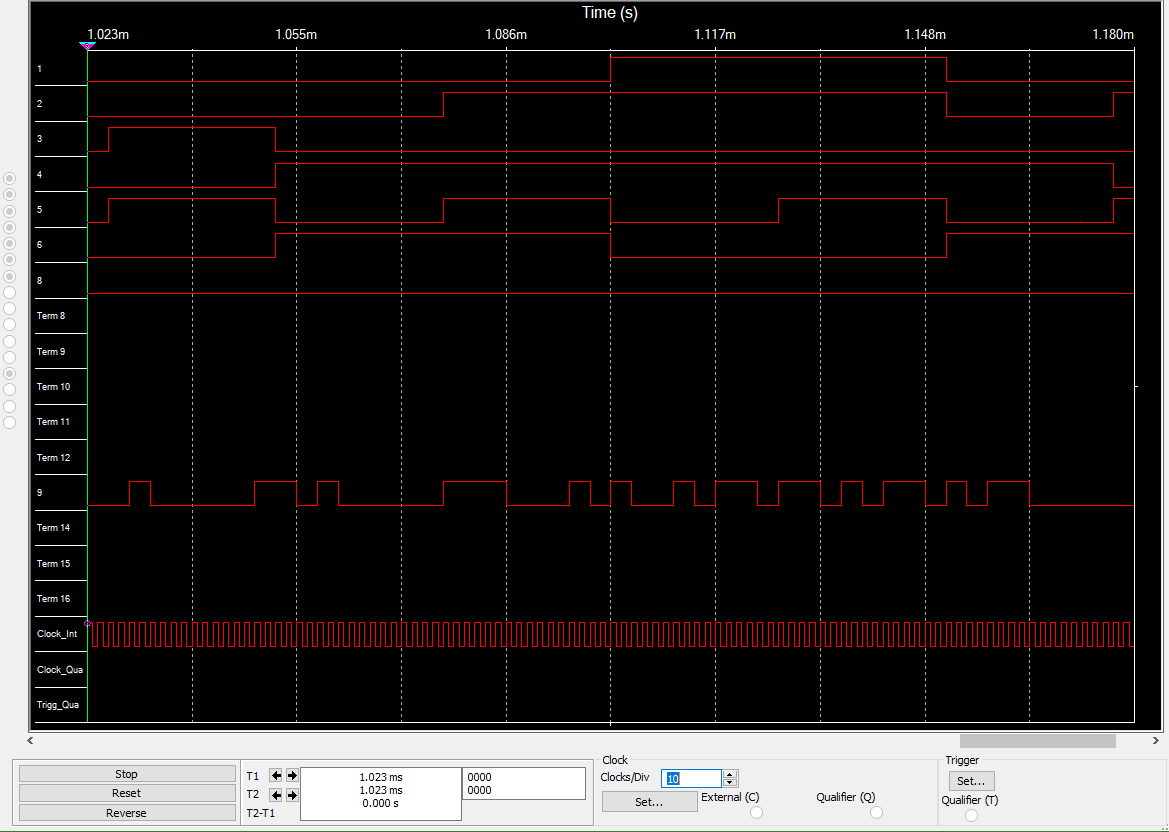
\includegraphics[width=0.75\textwidth]{images/adc_logic_analyzer.png}
    \caption{Resumen temporal en el analizador lógico: bus paralelo del ADC en el punto G (canales 1 a 8), trama digital
             serie en el punto H (canal 9) y reloj interno de sincronismo.}
    \label{fig.ej4:adc_logic_analyzer}
\end{figure}

El análisis de las señales registradas permite observar:
\begin{itemize}
    \item \textbf{Punto G (Canales 1 a 8, bus paralelo $D_0$ a $D_7$):} Representa la palabra binaria cuantizada a la
          salida del ADC. Las líneas $D_0$ a $D_2$ (bits de menor peso o LSBs) conmutan con alta frecuencia debido a su
          resolución de pocos milivolts ante las pendientes de la señal analógica. En contraposición, las líneas $D_5$ a
          $D_7$ (bits de mayor peso o MSBs) presentan transiciones estables y de menor cadencia, describiendo el ciclo
          fundamental de la onda senoidal de entrada de $1\,\unit{\kilo\hertz}$. Las actualizaciones del bus ocurren de
          forma sincrónica en cada flanco de muestreo del pulso SOC ($T_s = 25\,\unit{\micro\second}$).
    \item \textbf{Punto H (Canal 9, terminal Y):} Muestra la trama digital serie resultante a la salida del multiplexor
          $U_2$. El barrido de las entradas de selección A, B y C del multiplexor a través del generador de palabras
          recorre secuencialmente las líneas $D_0$ a $D_7$ durante el período de muestreo, conformando un flujo serie de
          pulsos lógicos binarios de duración constante $T_b = 3{,}125\,\unit{\micro\second}$.
    \item \textbf{Canal de reloj (`Clock\_Int`):} Registra la base de tiempos del analizador con un ajuste de 10 clocks
          por división, verificándose la estabilidad de los niveles lógicos y la sincronía entre la palabra paralela y
          la trama serie transmitida.
\end{itemize}

  \FloatBarrier
  \chapter{Conclusiones}
\label{sec.ej4:conclusiones}

El desarrollo de las simulaciones en NI Multisim permitió comprobar de manera práctica los conceptos fundamentales
de muestreo, recuperación y digitalización de señales establecidos en la consigna:

\begin{itemize}
    \item \textbf{Validación del Teorema de Nyquist:} Se comprobó que para una señal analógica de $10\,\unit{\kilo\hertz}$,
          una tasa de muestreo de $f_s = 40\,\unit{\kilo\hertz}$ satisface holgadamente la condición $f_s \ge 2 f_{\max}$.
          La banda de guarda resultante de $20\,\unit{\kilo\hertz}$ entre la banda base y la primera réplica lateral
          posibilitó la reconstrucción limpia de la onda senoidal mediante el filtro pasabajos de $10\,\unit{\kilo\hertz}$.

    \item \textbf{Expansión espectral y modulación de pulsos:} Se verificó por FFT que el muestreo expande el contenido
          espectral hacia frecuencias superiores mediante réplicas periódicas centradas en $n f_s \pm f_m$. El proceso
          físico responde a una modulación PAM natural donde la amplitud instantánea de los pulsos sigue la forma de la
          modulante, actuando cada armónico del tren como una portadora independiente.

    \item \textbf{Efecto de Aliasing:} Al reducir la tasa de muestreo a $15\,\unit{\kilo\hertz}$, se violó el criterio
          de Nyquist, generando una componente espuria en la frecuencia alias de $|15 - 10|\,\unit{\kilo\hertz} = 5\,\unit{\kilo\hertz}$.
          Al encontrarse dentro de la banda de paso del filtro de $10\,\unit{\kilo\hertz}$, dicha componente se superpuso
          con la fundamental, produciendo una distorsión irreversible caracterizada por un batido de $200\,\unit{\micro\second}$
          en el osciloscopio y dos rayas prominentes en la FFT.

    \item \textbf{Cuasi-muestreo sin componente continua:} El ensayo con portadora bipolar de media nula ($a_0 = 0$)
          demostró que la presencia de la modulante en banda base depende estrictamente del término continuo de la llave
          conmutadora. Sin continua, el sistema opera como un modulador balanceado DSB-SC; la energía se desplaza a las
          bandas laterales y la salida del filtro pasabajos se anula ($0\,\unit{\volt}$), requiriendo demodulación
          sincrónica para su recuperación.

    \item \textbf{Codificación PCM y serialización:} La simulación del ADC de 8 bits con fondo de escala de $2\,\unit{\volt}$
          arrojó un paso de cuantización de $7{,}8125\,\unit{\milli\volt}$. En el analizador lógico se constató la
          sincronía entre las 8 líneas del bus paralelo (punto G) y la trama binaria serie en la salida del multiplexor
          (punto H), alcanzando una tasa de transmisión de $320\,\unit{\kilo\bit\per\second}$ con duración de bit de
          $3{,}125\,\unit{\micro\second}$.
\end{itemize}

  \FloatBarrier

  \nocite{*}
  \printbibliography[heading=bibnumbered, title={Fuentes}]

\end{document}
